\documentclass[landscape, a0paper, final]{baposter}

\usepackage{blindtext}

\usepackage{amsmath}
\usepackage{amssymb}
\usepackage{amsfonts}

\usepackage{graphicx}
\usepackage{caption}
\usepackage{transparent}


\begin{document}
%% Define WZB colors
\definecolor{wzbGreen}{cmyk}{0.366,0,0.967,0.4}
\definecolor{wzbBlue}{cmyk}{0.983,0.293,0,0.29}
\definecolor{wzbMagenta}{cmyk}{0,0.69,0.272,0.38}

\begin{poster}{
  % --- General options ------------------------------------
  eyecatcher=true,  %% No funny picture to left
  background=none, %% white background
  % --- Box header settings --------------------------------
  headershape=rounded, %% shape box header
  headerborder=open, %% add border to header
  headerColorOne=wzbBlue, %% bg color header
  headershade=plain, %% no color gradient header
  % --- Box settings ---------------------------------------
  boxshade=none, %% no color gradient box content
  borderColor=wzbBlue, %% border color box content
  textborder=roundedright %% bottom shape box border
}
{
 %Eye Catcher, empty if option eyecatcher=no
}
{\sf A dictator's toolkit. How cooptation affects repression in autocracies}
{
\textsf{Replicated by} Dag Tanneberg, Berlin Social Science Center,
  Dept. `Democracy and Democratization', dag.tanneberg@wzb.eu%
}
{

\includegraphics[scale=.5]{./quareise.png}
}
\headerbox{\sf \color{white} Summary}{name=summary,column=0,row=0}{
  Dictatorships are mighty mean. They use different techniques of social
  control at the same time. Therefore, dictatorship differ on how mean
  they are, but not if.
}
\headerbox{\sf \color{white} Materials and Methods}{name=methods,column=0,below=summary}{
  \begin{align*}
    & \text{\sf Systematic:}\\
    & Y_i^\star \sim \mathcal{F}(\beta'\boldsymbol{x}_i, 1) \\
    & Y_i^\star = \beta'\boldsymbol{x}_i+\varepsilon_i \land 
      \varepsilon_i \sim \mathcal{F}_{L}(0, 1) \\
    & Y_i = m \iff \tau_{m-1} < Y_{i}^\star \le \tau_{m}~\forall~ 
      m \in \{1,\dots, M\} \\
    & \text{\sf Stochastic:} \\
    & Pr(Y_{i}=m|\boldsymbol{x}_i) = 
      Pr(\tau_{m-1} < Y_i^\star \le \tau_m | \boldsymbol{x}_i) \\
    & Pr(Y_{i}=m|\boldsymbol{x}_i) = 
      Pr(\tau_{m-1} < \beta'\boldsymbol{x}_i+\varepsilon_i \le \tau_m | 
        \boldsymbol{x}_i
      ) \\
    & Pr(\varepsilon_i \le \tau_{m} - \beta'\boldsymbol{x}_i) =
      \frac{1}{1+e^{-(\tau_{m}-\beta'\boldsymbol{x}_i)}}
  \end{align*}
}

\headerbox{\sf \color{white} First impression}{name=first,column=0,below=methods}{
  \begin{minipage}{\linewidth}
  \centering
  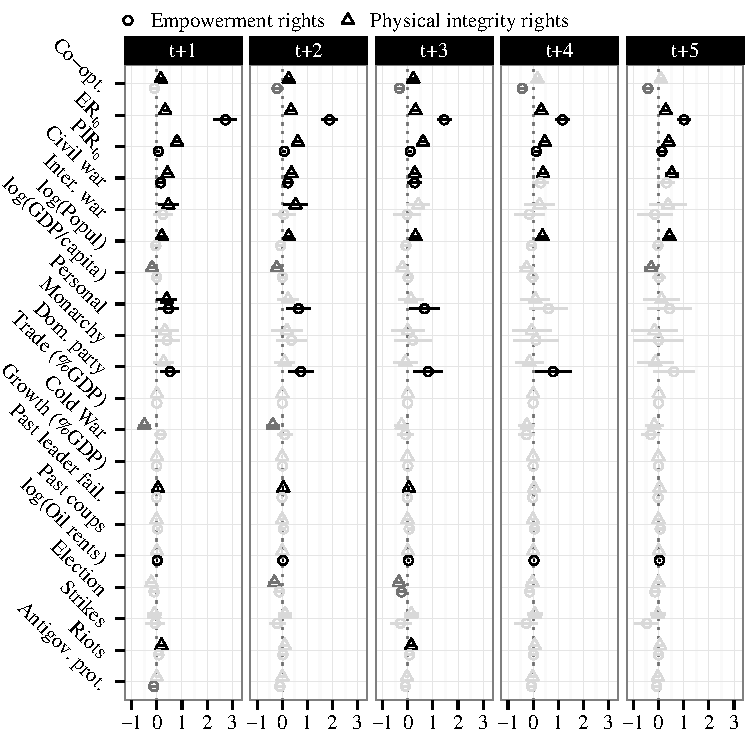
\includegraphics[width=3.1in]{/home/dag/Dropbox/Buero/Dissertation/2015/duke/classes/mle/termPaper/out/coefPlotOriginal.pdf}
  \end{minipage}
  The original results can be reproduced up to 2
  decimal places. Most often co-optation via 
  legislatures and political  parties tends to {\color{wzbBlue} reduce} 
  restrictions on empowerment rights. Simultaneously, it seems to 
  {\color{wzbMagenta} encourage} physical integrity violations.
}
\headerbox{\sf \color{white} Replication results}{name=results,column=1,span=2,row=0,textborder=rounded,bottomaligned=first}{
\begin{minipage}{.49\linewidth}
  \centering
  \includegraphics[width=3in]{/home/dag/Dropbox/Buero/Dissertation/2015/duke/classes/mle/termPaper/out/parallelRegrDevianceBonfP.pdf}
\end{minipage}
}

% \vfill
% \begin{minipage}{.49\linewidth}
%   \centering
%   \includegraphics[width=3in]{/home/dag/Dropbox/Buero/Dissertation/2015/duke/classes/mle/termPaper/out/parallelRegressionsPi_modified.pdf}
% \end{minipage}
% \vfill
% \begin{minipage}{.49\linewidth}
%   \centering
%   \captionof{figure}{Separation plots}
%   \includegraphics[width=3in]{/home/dag/Dropbox/Buero/Dissertation/2015/duke/classes/mle/termPaper/out/superSeperationER.pdf}
%   \captionof*{figure}{(a) Empowerment rights restrictions}
% \end{minipage}
% \vfill
% \begin{minipage}{.49\linewidth}
%   \centering
%   \includegraphics[width=3in]{/home/dag/Dropbox/Buero/Dissertation/2015/duke/classes/mle/termPaper/out/superSeparationPI.pdf}
%   \captionof*{figure}{(b) Physical integrity violations}
% \end{minipage}
% \hfill
% \begin{minipage}{.49\linewidth}
%   \centering
%   \captionof{figure}{Relative model fit}
%   \includegraphics[width=3in]{/home/dag/Dropbox/Buero/Dissertation/2015/duke/classes/mle/termPaper/out/aicDifferences.pdf}
% \end{minipage}
% }

\headerbox{\sf \color{white} Conclusions}{name=conclusions,column=3,row=0,textborder=roundedleft}{
  \blindtext
}

\headerbox{\sf \color{white} References}{name=references,column=3,below=conclusions,textborder=roundedleft}{
  \blindtext
}
\end{poster}
\end{document}